\documentclass{beamer}

\usecolortheme[light]{solarized}

\beamertemplatenavigationsymbolsempty


\usepackage{booktabs}
\usepackage{graphicx}
\usepackage{hyperref}
\usepackage{minted}
\usepackage{moresize}
\usepackage{standalone}
\usepackage{tcolorbox}
\usepackage{tikz}
\usepackage[normalem]{ulem}
\usepackage{xpatch}
\usepackage{fix-cm}

\xpatchcmd{\sout}
  {\bgroup}
    {\bgroup\def\ULthickness{2pt}}
      {}{}

\usetikzlibrary{calc, patterns}

\definecolor{twitter}{RGB}{64, 153, 255}
\definecolor{github}{RGB}{211, 211, 211}

\newcommand{\assetsfolder}{./assets}
\newcommand{\revisitresearchfolder}{$HOME/rsc/revisiting-axelrod-second}
\newcommand{\moranresearchfolder}{$HOME/rsc/axelrod-moran}
\newcommand{\mlresearchfolder}{$HOME/rsc/ml-paper}

\begin{document}

    \begin{frame}
        \begin{center}
            \Huge  
                Reproducible Science
                Reinforcement Learning
                Evolution

               \vfill

            \Large
               Vince: \href{https://twitter.com/drvinceknight}{@drvinceknight}\\
        \end{center}
    \end{frame}

    \begin{frame}
               \begin{columns}
                   \begin{column}{.45\textwidth}
                       \begin{center}
                       \includegraphics[height=3cm]{\assetsfolder/CUident_CMYK.eps}
                       \end{center}

                       \begin{center}
                       \includegraphics[height=3cm]{\assetsfolder/axelrod_logo.png}
                       \end{center}
                   \end{column}
                   \begin{column}{.45\textwidth}
                       \begin{center}
                       \includegraphics[height=3cm]{\assetsfolder/ssi-logo.png}
                       \end{center}

                       \pause
                       \begin{center}
                       \includegraphics[height=3cm]{\assetsfolder/flying_dog.jpg}
                       \end{center}
                   \end{column}
               \end{columns}
    \end{frame}

    \begin{frame}
        \begin{center}
            \fontsize{60}{70}\selectfont \(> 70\%\)
        \end{center}

        % Discuss this study in Nature that claims that >70% of scientific
        % studies are not reproducible
        % https://www.nature.com/news/1-500-scientists-lift-the-lid-on-reproducibility-1.19970
        % Discuss how this is field dependent of course and that in some cases
        % (for example in wet sciences) this is because details like how to or
        % whether to shake a jar of solution is included.
    \end{frame}

    \begin{frame}
        \HUGE
        \[
            \begin{bmatrix}
                0  &  1  &  0  &  0 \\
                1  & -1  &  1  &  0 \\
                0  &  1  & -1  &  1 \\
                0  &  0  &  1  &  0 \\
            \end{bmatrix}
        \]

        % Discuss ASMs: and what a mathematical proof is. Relate this to
        % "instructions". How mathematics as a  "science" is all about
        % reproducibility.
    \end{frame}

    \begin{frame}
        \begin{center}
            \Large
            \rotatebox{-45}{``The proof is left as an exercise for the reader."}
        \end{center}

        % But even in mathematics: we do not always do this well.
    \end{frame}

    \begin{frame}
        \begin{center}
            \fontsize{60}{70}\selectfont \(> 70\%\)
        \end{center}

        % Discuss the study by the SSI highlighting that 70% of research uses
        % software at some stage or another.
    \end{frame}

    \begin{frame}
        \begin{center}
            \href{https://twitter.com/ianholmes/status/288689712636493824?lang=en}{\includegraphics[width=.7\textwidth]{\assetsfolder/please-download-the-postdoc-tweet.png}}
        \end{center}
    \end{frame}

    \begin{frame}
        \begin{center}
            \href{https://twitter.com/betatim/status/1004077975233552385}{\includegraphics[width=.7\textwidth]{\assetsfolder/ms-github-importance-of-archiving-tweet.png}}
        \end{center}
    \end{frame}

    \begin{frame}
        \begin{center}
            \href{https://twitter.com/JamesCampbell95/status/996419422951825410}{\includegraphics[width=.7\textwidth]{\assetsfolder/blockchain-instead-of-archiving-tweet.png}}
        \end{center}
    \end{frame}

    \begin{frame}
        \begin{center}
            \href{https://twitter.com/legogradstudent/status/979776951517876225}{\includegraphics[width=.7\textwidth]{\assetsfolder/just-use-git-tweet.png}}
        \end{center}
    \end{frame}

	\begin{frame}
		\begin{center}
			\begin{tikzpicture}

				\node [font=\large, draw] (technology) at (-4, 4.5) {Technology};
				\node [font=\large, draw] (culture) at (4, 3.5) {Culture};

				\draw [very thick] (0, 0) -- (0, 6);
				\draw [very thick] (-2, 0) -- (2, 0);

				\draw [very thick] (-4, 6.5) -- (4, 5.5);
				\draw [very thick] (-4, 6.5) -- (technology);
				\draw [very thick] (4, 5.5)  -- (culture);
			\end{tikzpicture}
		\end{center}
	\end{frame}

	\begin{frame}
	   \begin{center}
		   \includegraphics[height=6cm]{\assetsfolder/ssi-logo.png}

			\url{https://www.software.ac.uk/}
	   \end{center}
	\end{frame}

	\begin{frame}
	   \begin{center}
		   \includegraphics[height=7cm]{\assetsfolder/UKRSE-logo.png}

			\url{http://rse.ac.uk/}
	   \end{center}
	\end{frame}

	\begin{frame}
	   \begin{center}
		   \includegraphics[width=8cm]{\assetsfolder/the-carpentries-logo.pdf}

			\url{https://carpentries.org/}
	   \end{center}
	\end{frame}

	\begin{frame}
	   \begin{center}
           \includegraphics[width=6cm]{\assetsfolder/joss-logo.png}

			\url{http://joss.theoj.org/}
	   \end{center}
	\end{frame}

	\begin{frame}
		\Huge
		\begin{center}
			\textit {For example...}
		\end{center}
	\end{frame}

	\begin{frame}
		\begin{center}
			\includegraphics[width=.7\textwidth]{\assetsfolder/lizard-tweet.png}
		\end{center}
		\begin{center}
			\pause
			\includegraphics[width=.35\textwidth]
			{\assetsfolder/lizard-cooperation.jpg}
		\end{center}

	\end{frame}

	\begin{frame}
		\fontsize{74}{65}\selectfont
		\begin{center}
			\(
				\begin{pmatrix}
					3 & 0\\
					5 & 1
				\end{pmatrix}
			\)
		\end{center}
	\end{frame}

	\begin{frame}[fragile]{}
		\begin{columns}
			\begin{column}{.4\textwidth}
				\begin{center}
					\includegraphics[width=.8\textwidth]{\assetsfolder/Axelrod.jpg}
					\\
					Robert Axelrod
				\end{center}
			\end{column}
			\pause
			\begin{column}{.6\textwidth}
				\begin{minted}[fontsize=\scriptsize]{python}
>>> import axelrod as axl

>>> players = (axl.TitForTat(),
...            axl.Cooperator())
>>> axl.Match(players, turns=5).play()
[(C, C), (C, C), (C, C), (C, C), (C, C)]

>>> players = (axl.TitForTat(),
...            axl.Defector())
>>> axl.Match(players, turns=5).play()
[(C, D), (D, D), (D, D), (D, D), (D, D)]

>>> players = (axl.TitForTat(),
...            axl.Alternator())
>>> axl.Match(players, turns=5).play()
[(C, C), (C, D), (D, C), (C, D), (D, C)]

				\end{minted}
			\end{column}
		\end{columns}
\end{frame}

	\begin{frame}
	\Huge
		\begin{center}
		TODO: Sacrifice kitten.
		\end{center}
	\end{frame}


    \begin{frame}
        \begin{center}
            \includegraphics[width=.7\textwidth]{\assetsfolder/axelrod-tweet.png}
        \end{center}
    \end{frame}

    \begin{frame}
        \begin{center}
            \fontsize{60}{70}\selectfont \(59\)
        \end{center}
    \end{frame}

\begin{frame}[fragile]{}
    \begin{minted}{fortran}
      FUNCTION K92R(J,M,K,L,R, JA)
    C BY ANATOL RAPOPORT
    C TYPED BY AX 3/27/79 (SAME AS ROUND ONE TIT FOR TAT)
    c replaced by actual code, Ax 7/27/93
    c  T=0
    c   K92R=ITFTR(J,M,K,L,T,R)
      k92r=0
      k92r = j
    c test 7/30
    c   write(6,77) j, k92r
    c77   format(' test k92r. j,k92r: ', 2i3)
      RETURN
      END
        \end{minted}
\end{frame}

\begin{frame}[fragile]{}

    \begin{center}
        \begin{minipage}{0.8\textwidth}
            \begin{minted}[fontsize=\Huge]{python}
import axelrod_fortran
            \end{minted}
        \end{minipage}
    \end{center}
\end{frame}

    \begin{frame}
        \begin{center}
            \scalebox{.8}{
                \documentclass{standalone}
\usepackage{tikz}
\usetikzlibrary{calc, shapes, patterns}

\begin{document}
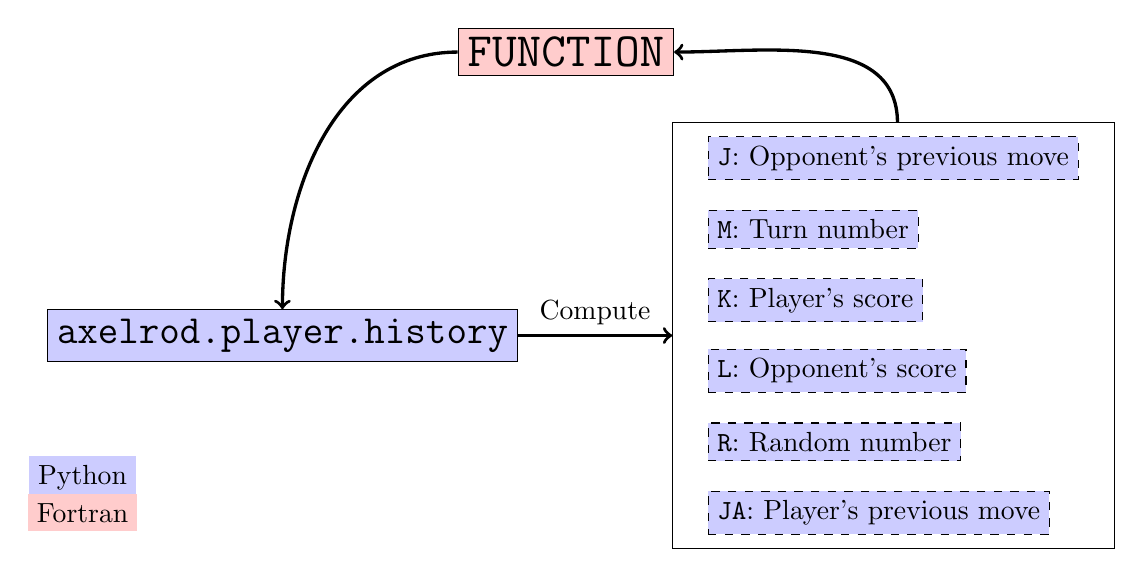
\begin{tikzpicture}[scale=.9]
    \node (axelrod_player) at (0, 0) 
        [draw, fill=blue!20, right] 
        {\Large \texttt{axelrod.player.history}};

    \node (fortran_function) at ($(axelrod_player) + (4, 4)$) 
        [draw, fill=red!20] 
        {\LARGE \texttt{FUNCTION}};

    % Computations
    \node (opp_previous_move) at ($(axelrod_player) + (6, 2.5)$) 
        [draw, fill=blue!20, dashed, right] 
        { \texttt{J}: Opponent's previous move};
    \node (current_move_number) at ($(axelrod_player) + (6, 1.5)$) 
        [draw, fill=blue!20, dashed, right] 
        { \texttt{M}: Turn number};
    \node (player_score) at ($(axelrod_player) + (6, .5)$) 
        [draw, fill=blue!20, dashed, right] 
        { \texttt{K}: Player's score};
    \node (opponent_score) at ($(axelrod_player) + (6, -.5)$) 
        [draw, fill=blue!20, dashed, right] 
        { \texttt{L}: Opponent's score};
    \node (random_number) at ($(axelrod_player) + (6, -1.5)$) 
        [draw, fill=blue!20, dashed, right] 
        { \texttt{R}: Random number};
    \node (player_previous_move) at ($(axelrod_player) + (6, -2.5)$) 
        [draw, fill=blue!20, dashed, right] 
        { \texttt{JA}: Player's previous move};


    \draw ($(opp_previous_move.east) + (.5, .5)$) 
                rectangle 
          ($(player_previous_move.west) + (-.5, -.5)$);

      \draw [very thick, ->] 
          (axelrod_player.east) -- node [above] {Compute} 
          ($(axelrod_player) + (5.5, 0)$);

      \draw (12, 3) edge[out=90, in=0, ->, very thick] 
          (fortran_function);
      \draw (fortran_function) edge[out=180, in=90, ->, very thick] 
          (axelrod_player);

    \node at (.5, -2) [fill=blue!20] {Python};
    \node at (.5, -2.5) [fill=red!20] {Fortran};
\end{tikzpicture}
\end{document}

            }
        \end{center}
    \end{frame}

    \begin{frame}
        \begin{center}
            \includegraphics[width=.9\textwidth]{\revisitresearchfolder/assets/original_tournament_rankings_all_approaches.pdf}
        \end{center}
    \end{frame}

    \begin{frame}
        \begin{center}
            \includegraphics[width=.9\textwidth]{\revisitresearchfolder/assets/original_tournament_with_extra_strategy_ranks_vs_library_ranks.pdf}
        \end{center}
    \end{frame}

    \begin{frame}
        \begin{center}
            \includegraphics[width=.7\textwidth]{\revisitresearchfolder/assets/full_tournament_pairwise_cooperation_rates.pdf}
        \end{center}
    \end{frame}

    \begin{frame}
        \begin{center}
            \textbf{Resistance}
            \includegraphics[height=.4\textheight]{\assetsfolder/moran_process_resistance.pdf}\\

            \textbf{Invasion}
            \includegraphics[height=.4\textheight]{\assetsfolder/moran_process_invasion.pdf}
        \end{center}
    \end{frame}


    \begin{frame}
        \scalebox{.7}{
            \input{\mlresearchfolder/assets/fsm.tex}
        }
    \end{frame}

\begin{frame}[fragile]{}

    \begin{center}
        \begin{minipage}{0.8\textwidth}
            \begin{minted}[fontsize=\Huge]{python}
import axelrod_dojo
            \end{minted}
        \end{minipage}
    \end{center}
\end{frame}


    \begin{frame}
        \begin{center}
            \scalebox{.7}{
                \input{\moranresearchfolder/tex/fsm_one.tex}
            }
        \end{center}
    \end{frame}


    \begin{frame}
        \begin{center}
            \includegraphics[height=.8\textheight]{./assets/hunger-games-hand-gesture.eps}


            \tiny
            \vfill
            \flushright{Image made by \url{http://www.freepik.com} from
            \url{https://www.flaticon.com} is licensed by CC BY 3.0}
        \end{center}
    \end{frame}


    \begin{frame}
        \scriptsize
        \begin{center}
            \textbf{Invasion (\(N=14\))}\\

            \input{\moranresearchfolder/tex/summary_top_14_invade.tex}
        \end{center}
    \end{frame}

    \begin{frame}
        \scriptsize
        \begin{center}
            \textbf{Resistance (\(N=14\))}\\

            \input{\moranresearchfolder/tex/summary_top_14_resist.tex}
        \end{center}
    \end{frame}


    \begin{frame}
        \begin{center}
            \includegraphics[width=.9\textwidth]{\assetsfolder/tf1_transitive_fingerprint.pdf}
        \end{center}
    \end{frame}

    \begin{frame}
        \begin{columns}
            \begin{column}{.6\textwidth}
                \begin{center}
                    \scalebox{.49}{
                        \input{\moranresearchfolder/tex/fsm_one.tex}
                    }
                \end{center}
            \end{column}

            \begin{column}{.4\textwidth}
                \small
                \begin{tabular}{ll}
                    \toprule
                    TF1 \#1   & TF1 \#2\\
                    \midrule
                    \bf{1}: C & \bf{1}: C  \\
                    \bf{8}: C & \bf{8}: C  \\
                    \bf{5}: D & \bf{5}: D  \\
                    4: C      & 4: C  \\
                    4: C      & 4: C  \\
                    4: C      & 4: C  \\
                    4: C      & 4: C  \\
                    4: C      & 4: C  \\
                    \bottomrule
                \end{tabular}
            \end{column}
        \end{columns}
    \end{frame}


    \begin{frame}
        \Huge
        \begin{center}
            \only<1>{
                164
                }
            \only<2>{
                \sout{164}\; 211+
                }
        \end{center}
    \end{frame}


\begin{frame}
    \begin{footnotesize}
        \begin{tcolorbox}[colback=github,colframe=blue!40!black,title=
                Julie Rymer - \href{https://gitter.im/Axelrod-Python/Axelrod?at=591388592b926f8a6741435d}
                {@Chadys} - (10 May 2017):
    ]
                And I really wanted to thank you all, I discovered your project because of a
                course where we needed to participate in an open source project, and I had the
                occasion to compare the welcome me and my coworkers received here compared to
                other people from my class who worked on different project. And I've got to said
                you are awesome on that part and on the help your provide to newbies  I like
                your project so I'll try to continue to contribute now and then !
       \end{tcolorbox}
    \end{footnotesize}

   \begin{columns}
        \begin{column}{.35\textwidth}
            \begin{itemize}
                \item \href{https://twitter.com/NikoletaGlyn}{@NikoletaGlyn}
                \item \href{https://twitter.com/opcampbell}{@opcampbell}
                \item \href{http://marcharper.codes/}{marcharper.codes}
            \end{itemize}
        \end{column}
        \begin{column}{.65\textwidth}
            \begin{itemize}
                \item \href{https://github.com/Axelrod-Python/Axelrod}{github.com/Axelrod-Python/Axelrod}
                \item \href{https://gitter.im/Axelrod-Python/Axelrod}{gitter.im/Axelrod-Python/Axelrod}
                \item
                    \href{https://arxiv.org/abs/1707.06920}{arxiv.org/abs/1707.06920}
            \end{itemize}
        \end{column}
   \end{columns}

        \begin{center}
               \href{https://twitter.com/drvinceknight}{@drvinceknight}
        \end{center}

   \begin{columns}
        \begin{column}{.5\textwidth}
            \begin{itemize}
                \item
                    \href{https://www.software.ac.uk/}{software.ac.uk}
                \item
                    \href{http://rse.ac.uk/}{rse.ac.uk}
            \end{itemize}
        \end{column}
        \begin{column}{.5\textwidth}
            \begin{itemize}
            \item
                \href{https://carpentries.org/}{carpentries.org}
            \item
                \href{http://joss.theoj.org/}{joss.theoj.org}
            \end{itemize}
        \end{column}
    \end{columns}
\end{frame}


\end{document}
